% Version 2020-01-06
% update – 161114 by Ken Arroyo Ohori: made spacing closer to Word template throughout, put proper quotes everywhere, removed spacing that could cause labels to be wrong, added non-breaking and inter-sentence spacing where applicable, removed explicit newlines
% update – 010819 by Dennis Wittich: made spacing and font size closer to Word template, updated references and refernces style
% update – 042319 by Dennis Wittich: font size of captions set to 'small', first author names are shortened, hyphenation fixed
% update – 010620 by Dennis Wittich: Footnotes alignment set to left
% update - 151220 by Clement Mallet: Template adapted for single blind abstract submissions


\documentclass{isprs} % isprs class modified 23-04-2019 (Dennis Wittich)
\usepackage{subfigure}
\usepackage{setspace}
\usepackage{natbib}
\usepackage{cleveref}
\usepackage{booktabs}
\usepackage{geometry} % added 27-02-2014 Markus Englich
\usepackage{epstopdf}
\usepackage[labelsep=period]{caption}  % added 14-04-2016 Markus Englich - Recommendation by Sebastian Brocks
\usepackage[british]{babel} 
\usepackage[hang]{footmisc}
\def\footnotemargin{1em} % added 08-01-2020 Dennis Wittich

%\usepackage[authoryear]{natbib}
%\def\bibhang{0pt}

\geometry{a4paper, top=25mm, left=20mm, right=20mm, bottom=25mm, headsep=10mm, footskip=12mm} % added 27-02-2014 Markus Englich
%\usepackage{enumitem}

%\usepackage{isprs}
%\usepackage[perpage,para,symbol*]{footmisc}

%\renewcommand*{\thefootnote}{\fnsymbol{footnote}}
\captionsetup{justification=centering,font=normal} % thanks to Niclas Borlin 05-05-2016
\captionsetup[figure]{font=small} % added 23-04-2019 Dennis Wittich
\captionsetup[table]{font=small} % added 23-04-2019 Dennis Wittich

\begin{document}

\title{Geomorphological mapping of intertidal areas 
}
% Leave empty (\version{}) when submitting the abstract
\version{}

% KAO: Remove extra spacing
\author{
 M. Lu\textsuperscript{1}\thanks{Corresponding author}, 
 L. Groeneveld\textsuperscript{1}, 
 D. Karssenberg\textsuperscript{1},
 S. Ji\textsuperscript{3}, 
 R. Jentink\textsuperscript{2}, 
 E. Paree\textsuperscript{2},
 E. Addink\textsuperscript{1}}

% KAO: Remove extra newline
\address{
	\textsuperscript{1} Department of Physical Geography, Utrecht University, the Netherlands lumeng0312@gmail.com\\
	\textsuperscript{2} Rijkswaterstaat CIV, the Netherlands \\
	\textsuperscript{3} Department of remote sensing and information engineering, Wuhan University, China. \\
	}

% If the corresponding author is NOT the final author, always add a % space before the subsequent comma, i.e.
% first author name\textsuperscript{a,}\thanks{Corresponding author} , % second author name \textsuperscript{b}, etc.
% thanks to Niclas Borlin 05-05-2016


\commission{ZZ, }{YY} %This field is optional. If filled, XX and YY should be replaced by adequate numbers. See https://www2.isprs.org/commissions/
\workinggroup{XX/YY} %This field is optional.
\icwg{}   %This field is optional.


\keywords{Geomorphology, Inter-tidal flats, semantic segmentation, multi-dimensional, feature interpretation, OBIA, XGBoost}

\maketitle

%\saythanks % added 28-02-2014 Markus Englich

\section{Introduction}\label{Introduction}
 
% KAO: Sloppy spacing ensures non-overfull lines. Can be removed if this is not an issue.
\sloppy

\subsection{Background}
\label{sec:Introduction}
Spatiotemporal geomorphological mapping of intertidal areas is essential for understanding system dynamics and provides information for ecological conservation and management \citep{bouma2005zoute}. Ecological quality of intertidal areas is important because of the European Water Framework Directive and as they are designated as Natura 2000 areas, which is the implementation of the European bird directive and the European habitat directive. Mapping the geomorphology of intertidal areas is a considerable challenge mainly because spectral differences are oftentimes relatively small while transitions between geomorphological units are oftentimes gradual. Also, the intertidal areas are highly dynamic \citep{kleinhans2019tidal}. Surface water, saltmarsh, and tidal flats are relatively simple to distinguish but considerable challenges remain for distinguishing between different types of tidal flats, specifically, low and high dynamic shoal flats, sandy and silty low dynamic flats, and mega-ripple areas \citep{Douma2019}. In this study, we harness machine learning methods in automated geomorphological mapping and extend object-based methods with deep neural network-based semantic segmentation methods. We focus on distinguishing between 5 classes:  sandy low dynamic flats, silty low dynamic flats, mega-ripples, high dynamic shoal flats, and hard substrates. We evaluate the methods used with an extensive data set of visually interpreted photos.
%for multiple years.

\subsection{Objective}
%The objectives of this study are to 1) understand how temporal, spectral and geometric information, elevation, and contextual features contribute to the delineation of the tidal flats, 2)

The objectives of this study is to compare between the methods that are based on ensemble tree-based modeling on features of segments from classical OBIA vs. deep neural networks-based methods.
%, and a new method that integrates both approaches. 

\subsection{Impact}
This study is both application- and method-driven. It provides us with an in-depth understanding of features that contribute to tidal area classification and is expected to greatly improve the automation of the procedure and the prediction accuracy. We emphasise model interpretability and knowledge mining. By comparing and combining object-based and deep learning-based models, this study contributes to the integration of thus far largely separate approaches for semantic segmentation. 

\section{Methodology}\label{method}
 
The study is mainly developed in Western Scheldt, the Netherlands (\cref{fig:ws_o}), where a detailed manually delineated expert classification map is available. 
%We also conduct extensive evaluations in a study area with different geomorphological characters, Wadden Sea (\cref{fig:wadden}), to evaluate model generality. 
\Cref{fig:ws_o} (b) shows our classification scheme. Importantly, we distinguish between the sandy and silty areas within the shoal flat low dynamics (\cref{fig:xgb}). We used aerial imagery with red, green, and NIR bands (0.25 m resolution), DEM from laser altimeters (2 m resolution), and derived indices. Imagery and DEM are acquired within the same year and season. Two methods are developed and compared in terms of the priors integrated, model interpretability, and the prediction accuracy and patterns. The first method firstly applies OBIA (Object-based Image Analysis) for segmentation and then uses an emsemble tree-based method, XGBoost \citep{Chen:2016:XST:2939672.2939785}, for classification, this method is referred to (OBIA-XGB) in this study. The challenges of this method lie in the identification of the optimal spatial unit of objects. The second method applies an encoder-decoder deep neural network architectures, U-net \citep{ronneberger2015u}, for end-to-end classification. 

% leave out for this paper because we havent reached them. 

%Besides interpreting features extracted at activation layers, we apply channel-attention modules to integrate and understand the impacts of temporal, spectral features and DEM, and spatial attention modules with dilated convolutions and multi-scale network architectures for the contextual features. 

%Method (C) applies object-based image analysis to the segmented output from deep neural networks to integrate prior knowledge. 

%At last, we invest in applying generative modeling and image augmentation to enhance features at the pre-processing stage. Our preliminary results indicate the importance of geometric and contextual features and support our future developments. 

\begin{figure}
    \centering
    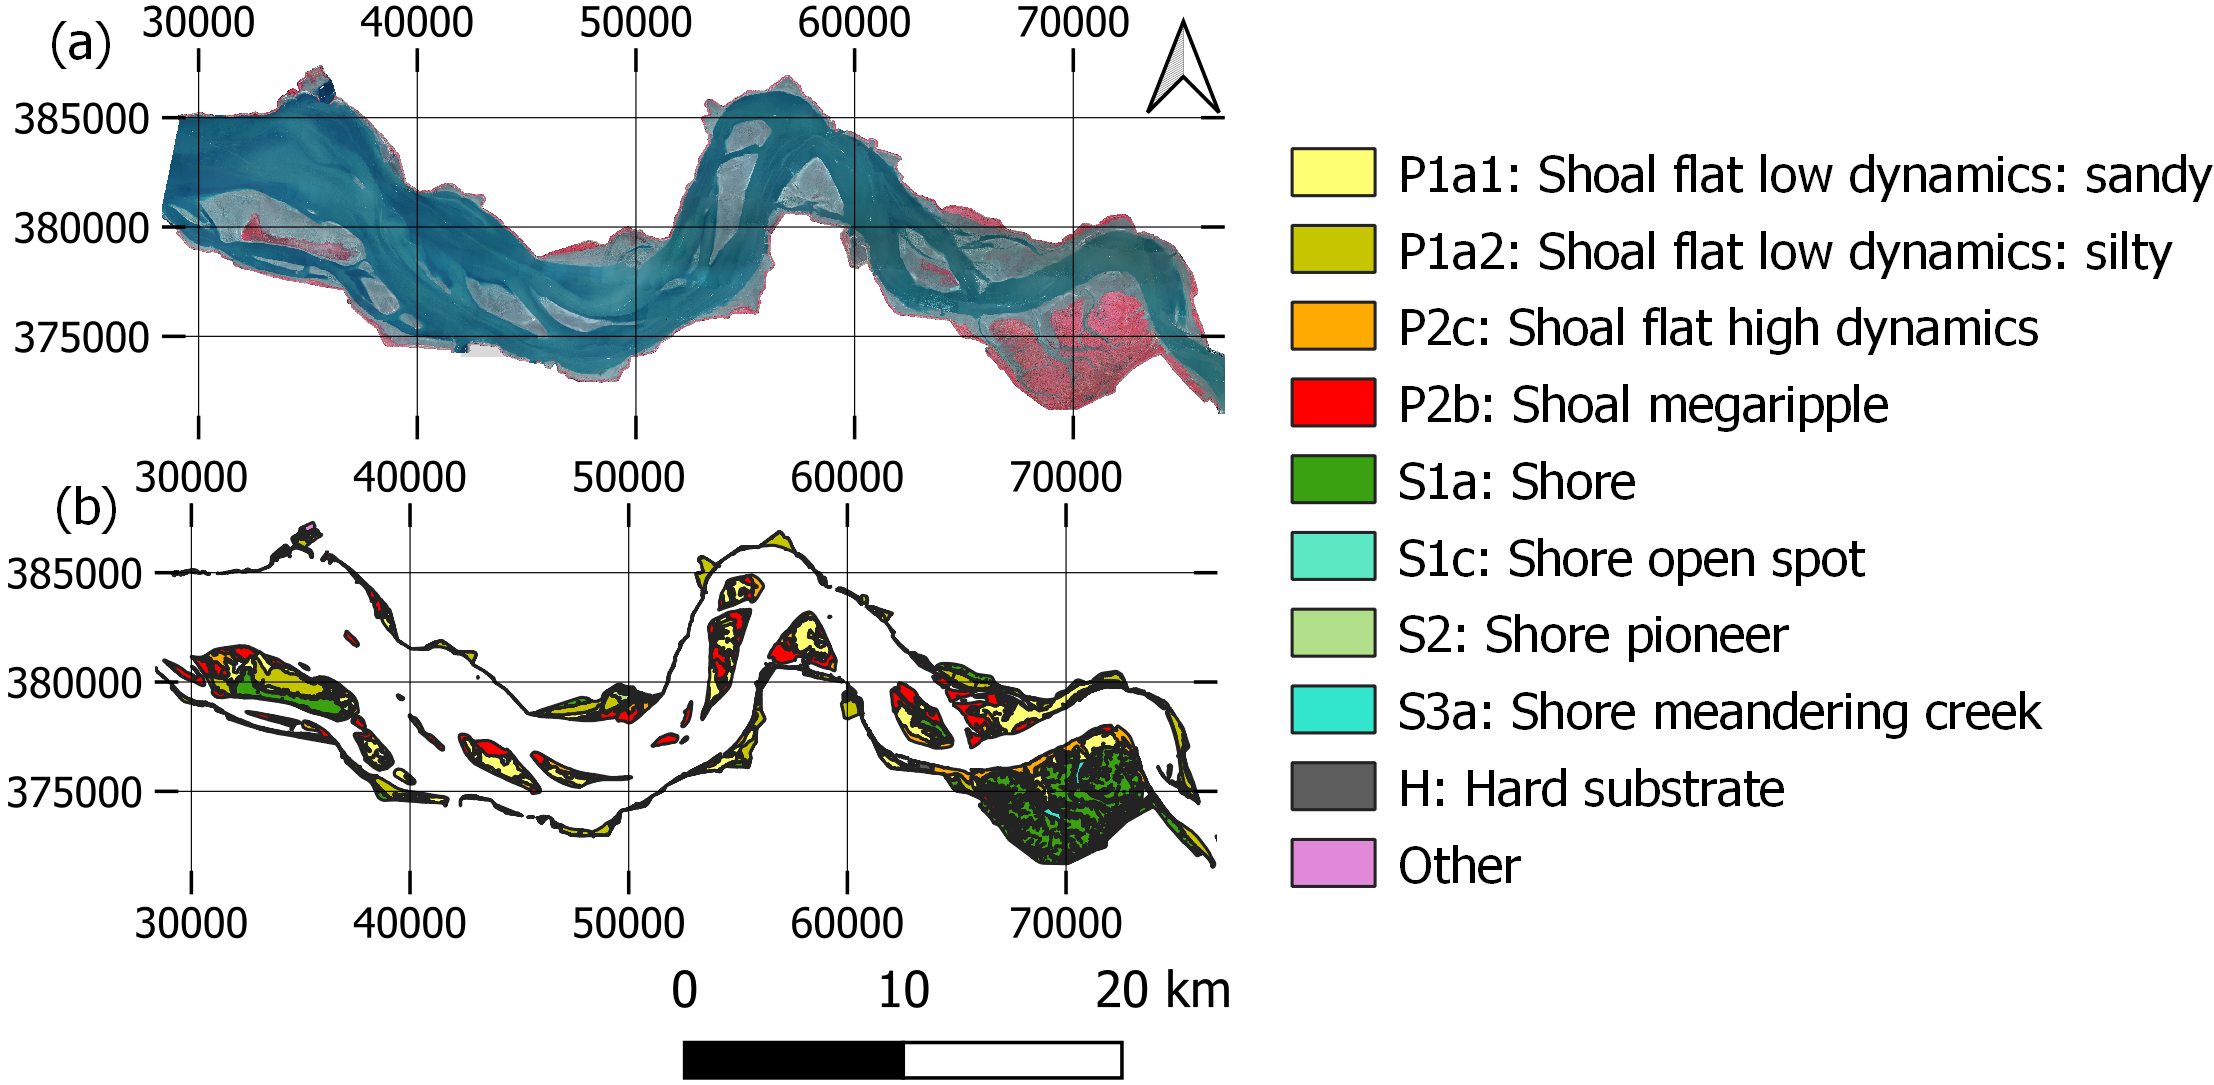
\includegraphics[scale=0.4]{figures/westernscheldt_overview.png}
    \caption{The Western Scheldt study area. Figure (a): false color aerial image with the red, blue, and Near-Infrared bands, 0.25 m resolution. Figure (b): the expert map and classification schemes.}
    \label{fig:ws_o}
\end{figure}

\begin{figure}[!h]
    \centering
    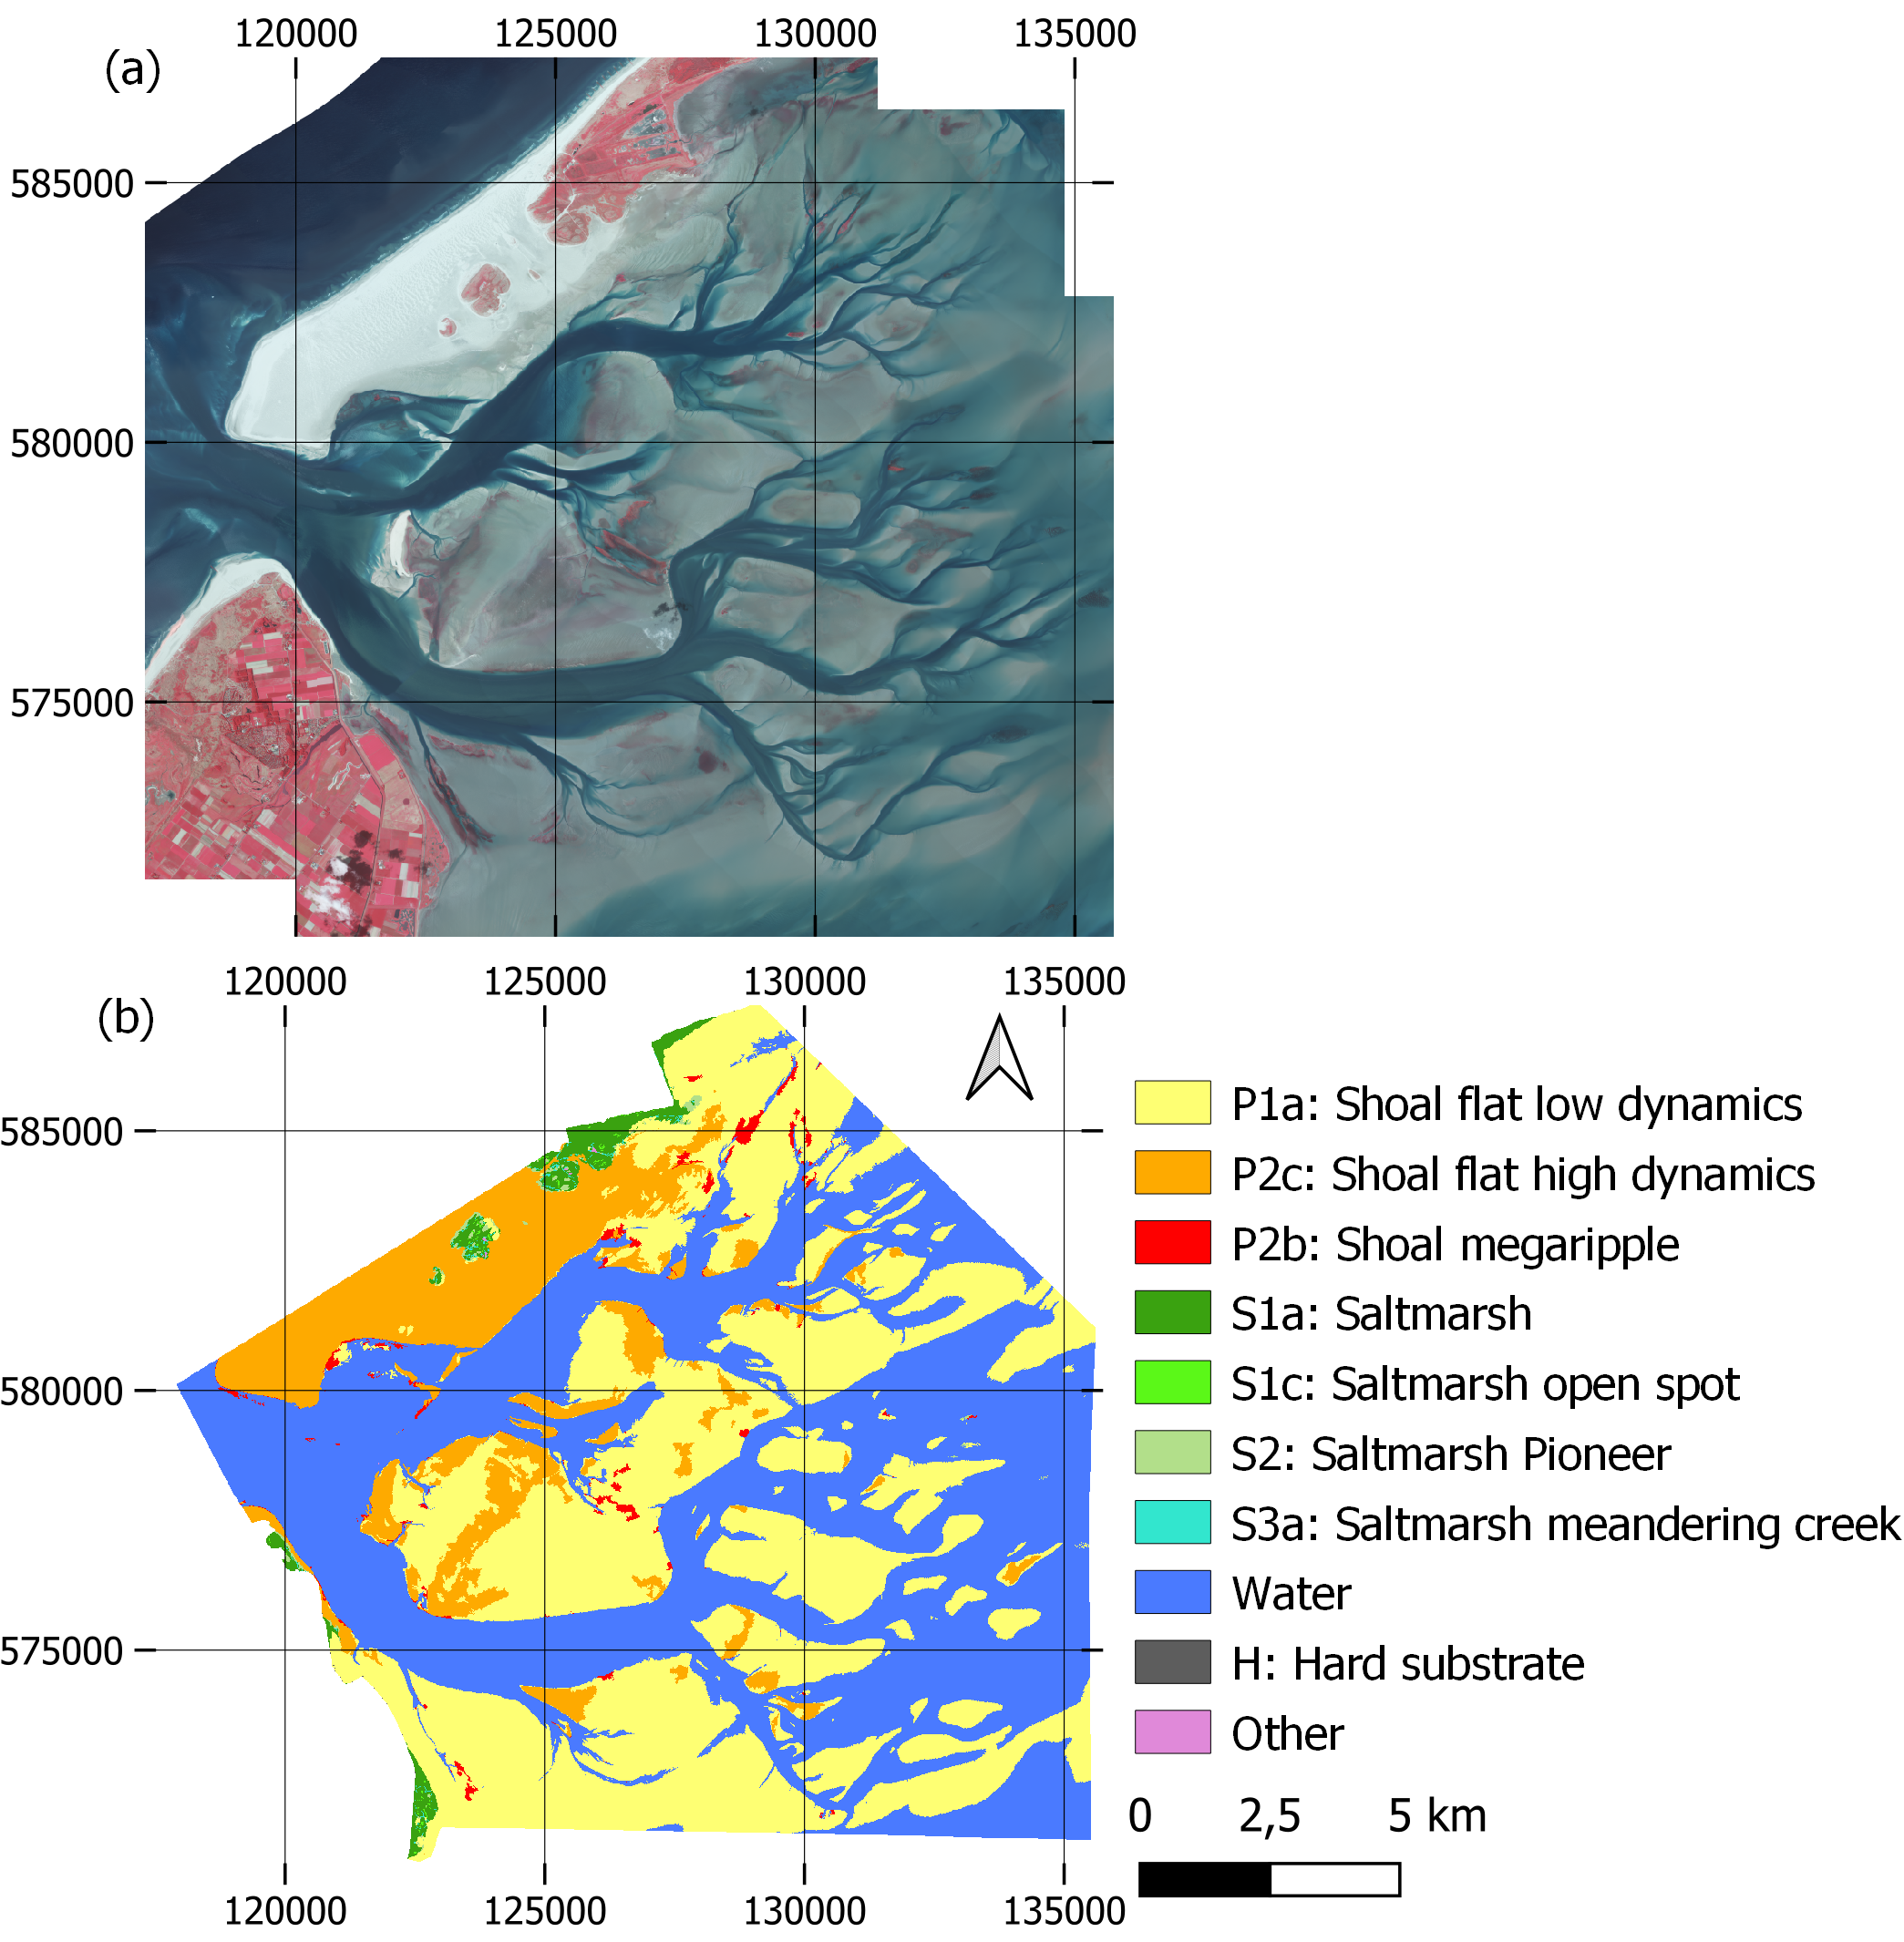
\includegraphics[scale=0.4]{figures/false_classificationvertical.png}
    \caption{(a): the Wadden Sea study area, visualised in false color with the red, green, and Near-Infrared bands of aerial images of 0.25 m resolution. (b): the classification schemes. The map is made by manually fine-tuning the result of an OBIA model. The model was developed in the Western Scheldt and adapted to make it more general. }
    \label{fig:wadden}
\end{figure}

\subsection{Preprocessing}

We focus on distinguishing between 5 classes and for convenience, we assign a code to each of them: 
\begin{itemize} 
\item P1a1: sandy low dynamic flats  
\item P1a2: silty low dynamic flats 
\item P2b:  mega-ripples
\item P2c: high dynamic shoal flats
\item H1: hard substrates
\end{itemize} 

For the definition of the classes please refer to \cite{Douma2019}. We also refer to the P1a1, P1a2, P2b, and P2c classes as the "P" class and the H1 class "H" class. The other classes (i.e. classes that do not belong to the P and H1 classes) are removed. 

We filtered out water by firstly using eCognition (Developer 9.4.0) to do segmentation, and then using the NDWI ($NDWI = \frac{green - NIR}{green + NIR}$) with a threshold of 0.44. Mega-ripples naturally consists of water. In this study, we also filtered out water in the P2b (mega-ripple) class to gain an initial understanding of the behaviour of machine learning models.   

\subsection{Sampling scheme}
\label{cv}

As the unit of method OBIA-XGB is OBIA segments and method U-net image pixels, we develop different sampling schemes for each of them. For method OBIA-XGB, it is necessary to develop a sampling scheme that accounts for the object size for the tree classifier. We evaluated two sampling schemes: 1) random sampling and 2) stratified sampling according to the size of OBIA segments. For 1), we used random under-sampling to sample the majority class(es), without replacement, to ensure the classes have balanced samples. For 2), we firstly divided the objects into 5 categories, cut at each 2nd, 4th, 6th, 8th, 10th percentiles of the object size of the minority class (i.e. class with the least number of objects). These percentiles are chosen so that the number of objects in these categories are similar. Within each category, 70\% of the objects form the training set and the rest forms the test set. Then within the training set of each category, random under-sampling is applied. 

For OBIA-XGB, we selected three tiles that are abundantly covered by the focused classes (i.e. P and H1 classes). For the method based on U-net, we selected 80 500 pixels $\times$ 500 pixels tiles for training (42 tiles) and validation (18 tiles). Three 4000 $\times$ 4000 tiles are used for testing (\cref{fig:tt}). 

\begin{figure}
    \centering
    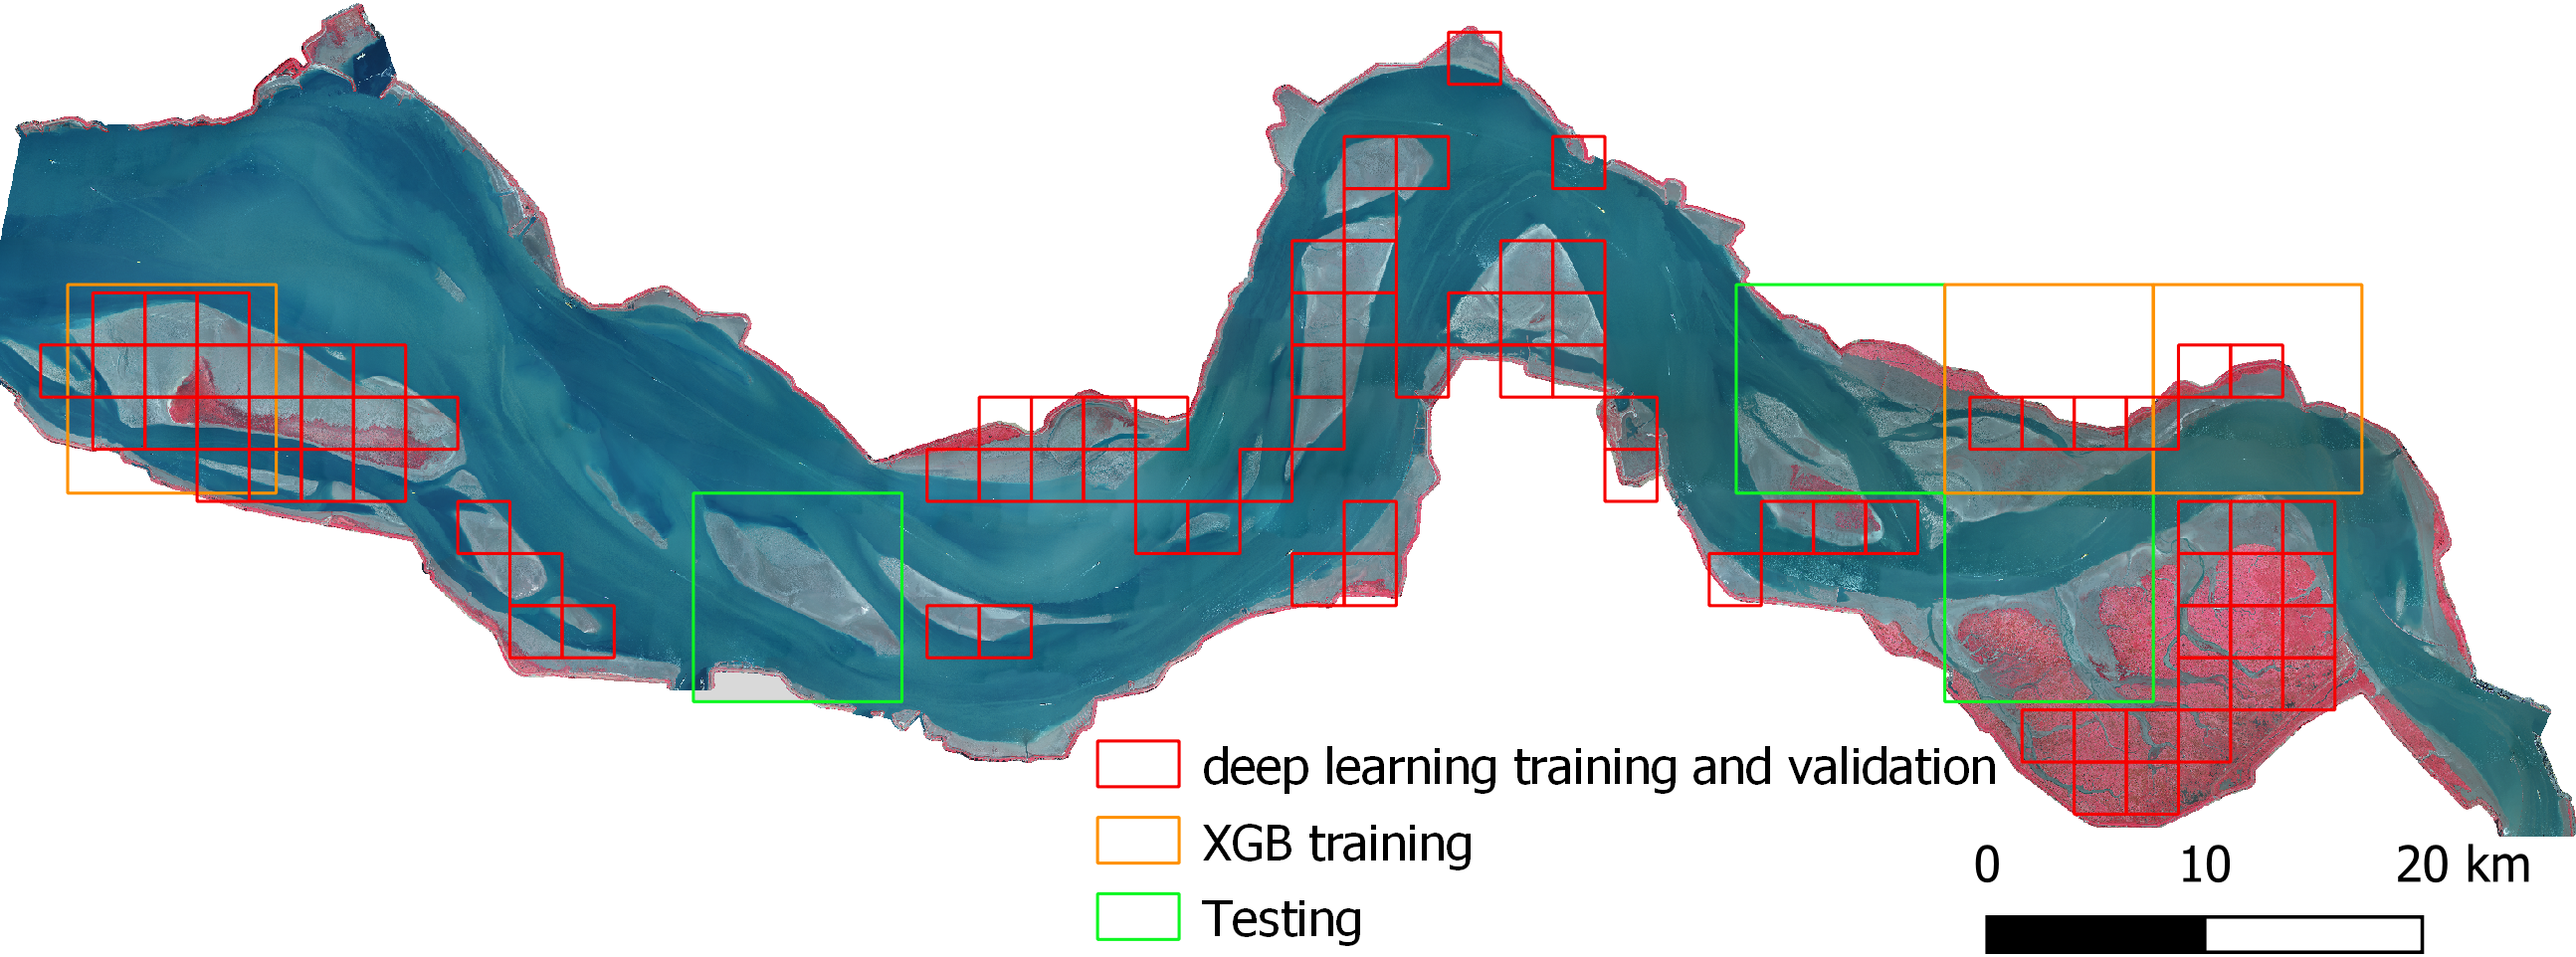
\includegraphics[scale = 0.3]{figures/train_test_tileOverview.png}
    \caption{Training, validation, and test areas used in Western Scheldt.}
    \label{fig:tt}
\end{figure}

\subsection{Accuracy assessment}

We focus on the precision (True Positives)/(True Positives + False Positives) and recall (True Positives)/(True Positives + True Negatives) as indicators of the prediction accuracy.  
%and additionally IoU (Intersect over Union) for (B). 
For method A, the precision and recall are weighted by the area size of each object for the final recall and precision. In addition, we present the precision and recall based on objects (i.e. not weighted by the area size). This serves to inspect how the objects with various sizes are identified.  

\section{Experiments}

\subsection{Method OBIA-XGB}

The inputs of the OBIA-XGB method are aerial imagery (with NIR, red, green bands) and DEM, as well as slope \citep{zevenbergen1987quantitative}, NDVI, and aspect (\citep{horn1981hill}) derived from eCognition. 

We firstly use eCognition for object segmentation at various spatial units. Then, we combine segmentation levels to get sub-object describing brighter and darker sub-objects features. We export the objects with in total 48 features describing the spectral and texture (using Harralick's grey level co-ocurrence matrices) features of objects and sub-objects.
%Lars: add details, which features and sub-features you exported. 

Then, to determine the optimal spatial unit for each class, we each time regroup the five classes into the "target class" and the "other class" and iterate over all the five classes. The XGBoost is applied to classify the OBIA calculated object features and select the best spatial unit for each class based on the prediction accuracy. 

We found no considerable differences in the optimal spatial unit for each class (will be described in \cref{sec:suo}, \cref{fig:overview}), therefore, we used a single optimal spatial unit for all classes. The identified optimal spatial unit is used for multi-class classification. The loss functions for the binary and multi-class classifications are respectively the \textit{logistic loss} and \textit{softmax} loss (i.e. a softmax activation followed by a cross-entropy loss). 

The hyperparameters we tuned for XGBoost are learning rate, maximun tree-depth, number of estimators, and the Lasso regularisation term $\alpha$, using 5-fold cross-validation. The modeling process using XGBoost and deep neural networks is implemented in the Python environment (version 3.6). 

\subsection{Method-based on U-net}

The input for the U-net is the aerial imagery, DEM, and derived slope \citep{horn1981hill}, NDVI and a Brightness layers. The slope was calculated in QGIS3.18 using the same Horn's formula \citep{horn1981hill} as in eCognition, and is expressed in degrees. The NDVI and brightness are calculated in Python. The Brightness is defined as $Brightness =  (NIR+red+green)/3$.
 
The loss functions we tested are categorical cross-entropy loss, IoU loss \citep{van2019deep}, FocalTverskyLoss \citep{abraham2019novel}, and Lovasz Hinge Loss \citep{berman2018lovasz}. In the end, we chose to use the IoU loss as it provides the best cross-validation results with the training set. The hyperparameters we tuned are learning rate, batch size, and image size. The image size tested are from $2^5$ (64) to $2^9$ (512) and is optimised at 128. The batch size tested are from 8 to 32 and is optimised at 16. The learning rate are tested with various scheduling, ranging from 0.0001 to 0.01 at various epochs. 
 

\section{Results}
\label{sec:results}

\subsection{Spatial unit optimisation for OBIA-XGB}
\label{sec:suo}

 \Cref{fig:overview} shows the precision and recall of different sampling schemes and cross-validation methods for the binary classification in the Western Scheldt study area. The stratified sampling greatly improves the prediction accuracy, comparing the cross validation between applying our stratified sampling (SS) scheme to random sampling of the objects (object).
 
  \begin{figure}[!h]
    \centering
    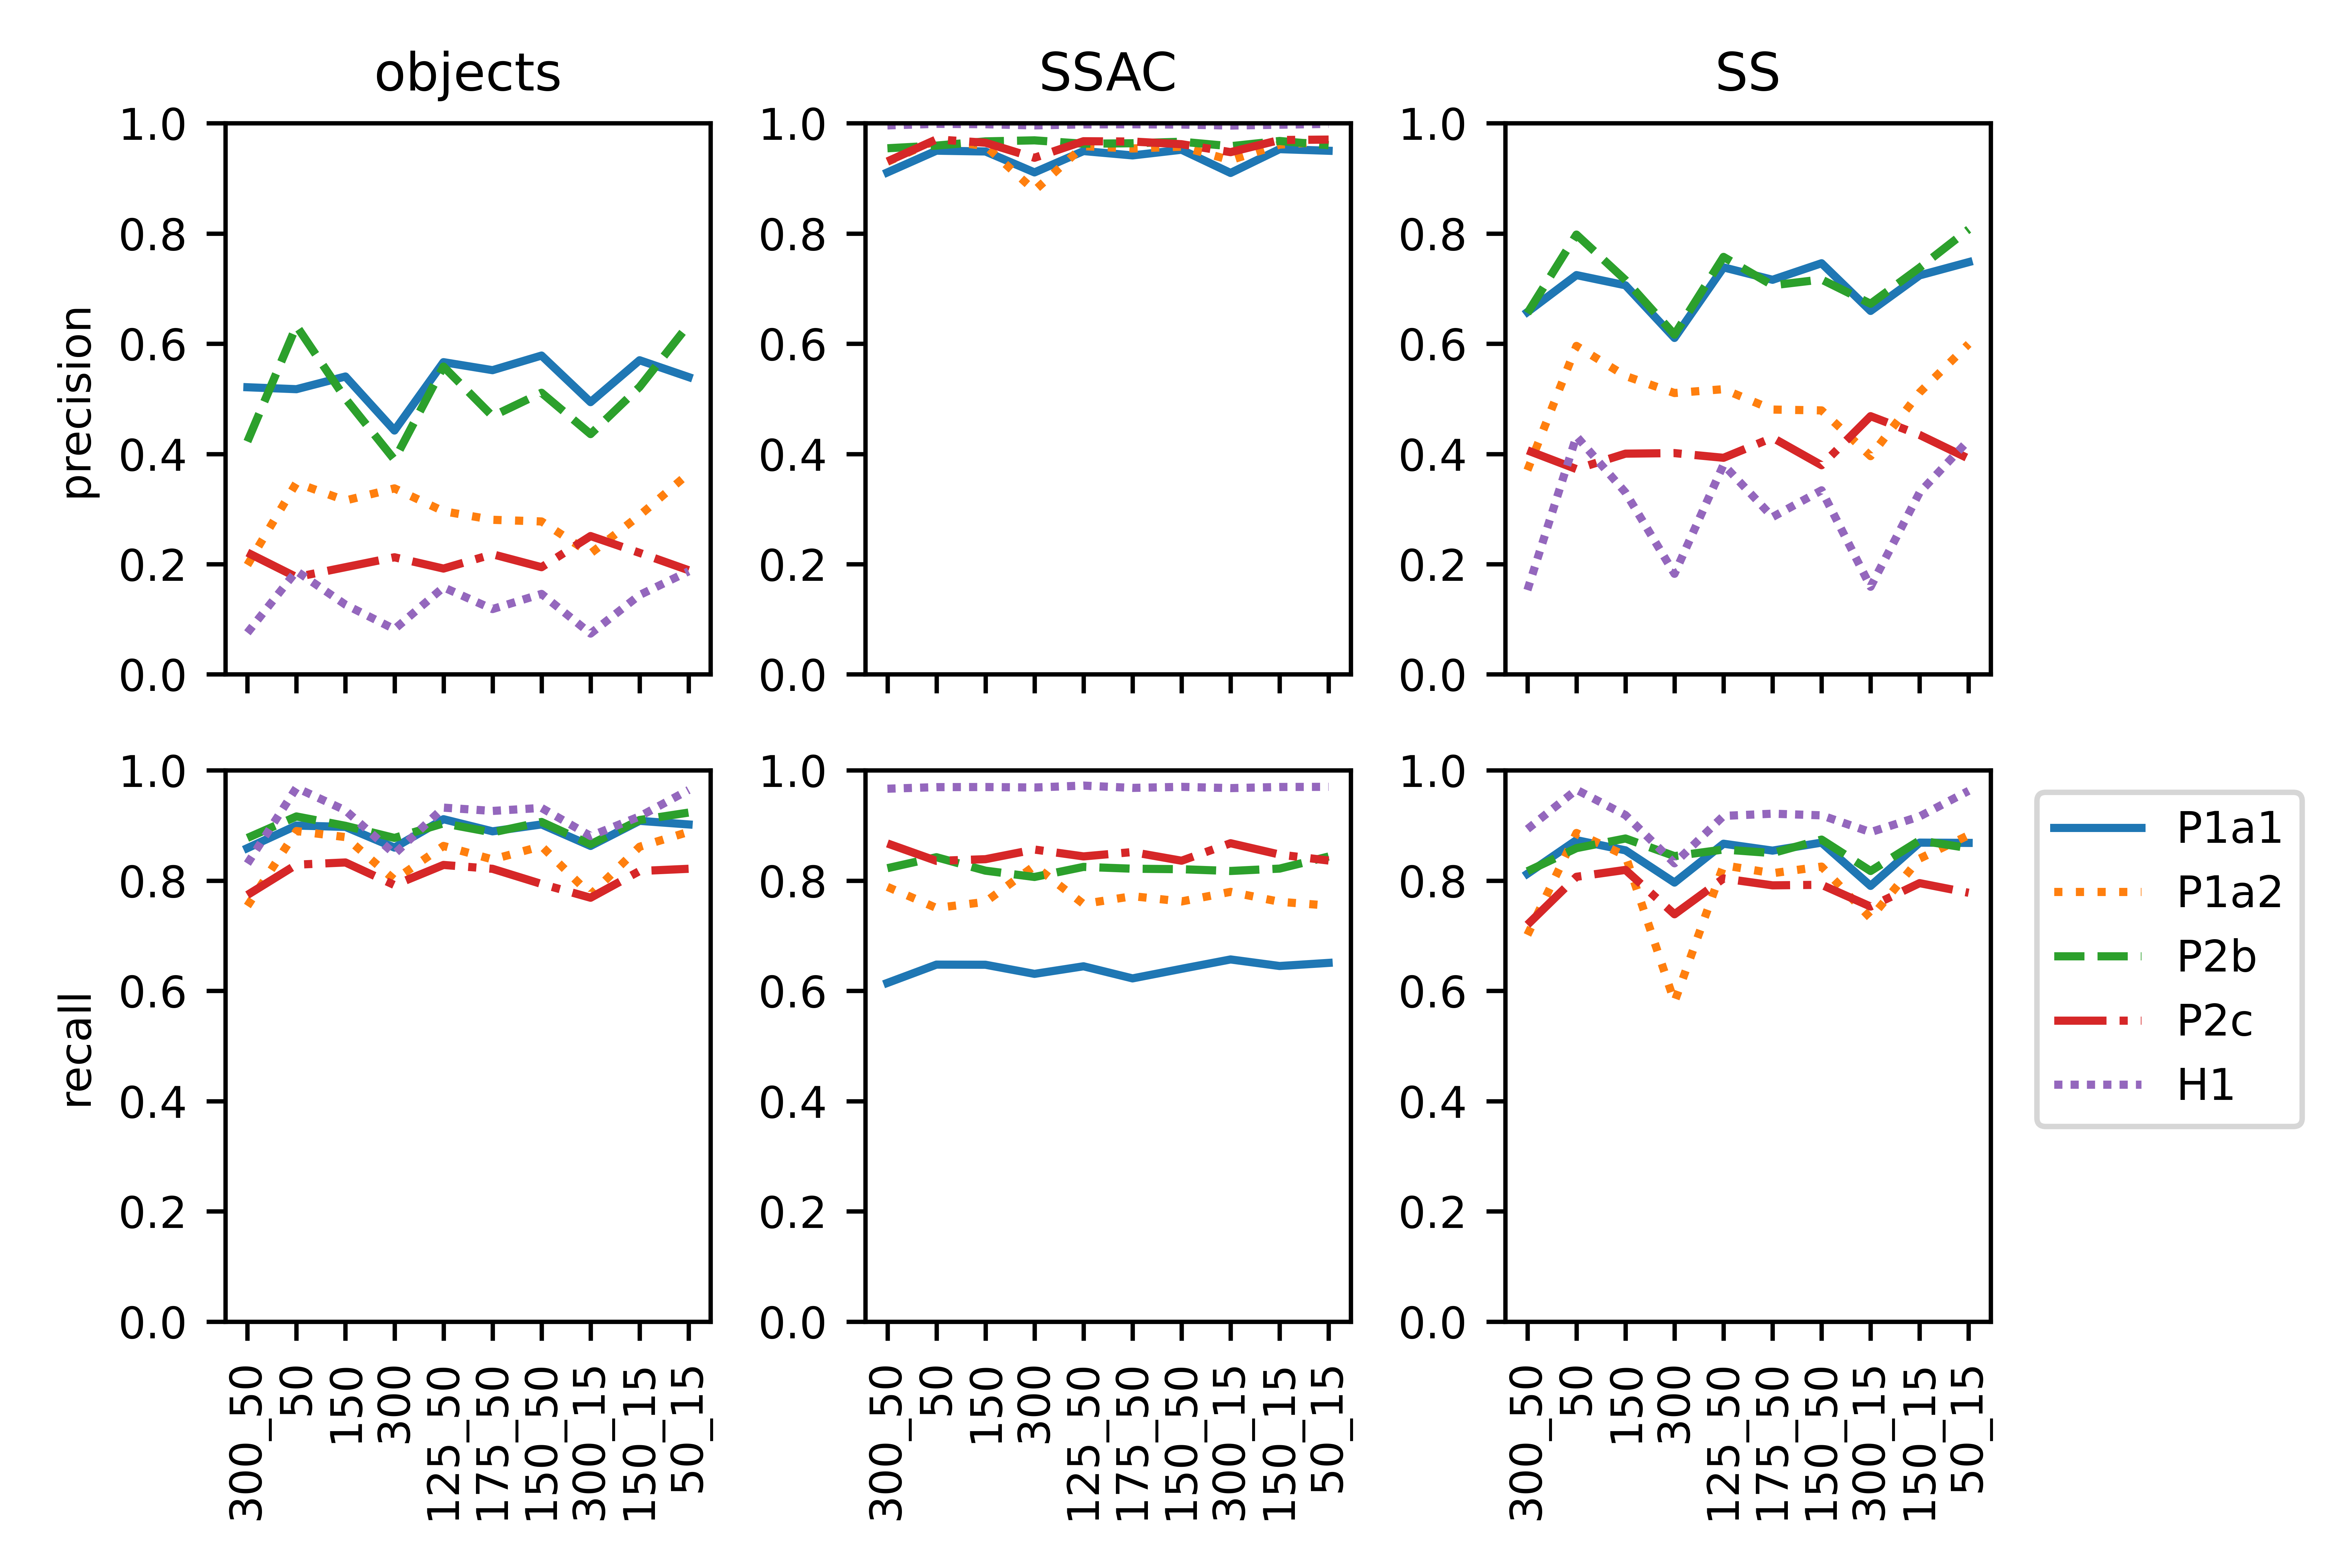
\includegraphics[width=\linewidth]{figures/overview_total.png}
    \caption{Cross-Validation results for all the classes, with the XGBoost classifier on OBIA objects. Objects: random sampling and cross-validation based on objects. SSAC: stratified-area sampling with area-weighted cross-validation results. SS: stratified-area sampling.}
    \label{fig:overview}
\end{figure}

 It could be observed that when using both stratified sampling and area-weighted cross-validation (SSAC), all the classes obtained a very high precision with each of the tested spatial unit, indicating that larger objects are better identified than the smaller objects. The recall remains high for the H class but is lower for the P classes, especially the P1a1. Compared to SS, which has a relatively high recall for all the classes but much lower and diverse precision for different spatial units and classes, it is found that objects with smaller sizes are more likely to mix with other classes, especially for the P1a1, P2c, and H class. As the SSAC shows homogeneous recall and precision between spatial units, to optimise the classification for small objects and ensure the highest model generality, we use SS to identify the optimal spatial unit. The optimal spatial unit identified for all classes are 50\_15 (object level 50, sub-object level 15).   
 
%the optimal spatial unit identified is 50 with sub-object level 15

\subsection{Prediction accuracy}
\subsubsection{Method OBIA-XGB}
The multi-class classification results for the method OBIA-XGB are shown in \cref{xgb_ss,xgb_ssac,fig:spxgb}. SSAC is used to indicate the performance and SS for indicating how well the smaller objects are classified. According to SSAC, the megaripple class obtained the highest precision, indicating the method OBIA-XGB is already promising in distinguishing it from other P classes and the H1 class. The sandy and silty low dynamic flats are also separated well. 

Comparing \cref{xgb_ss,xgb_ssac}, it is observed that small objects are classified best in the P2b and H1 classes but are less satisfying in P1a1, P1a2, and P2c. \Cref{fig:spxgb} shows that most of the objects are correctly classified, mis-classification mostly occur as classifying P1a1, P1a2 and P2b as H1, especially along some streams outlets or close to water. 
%\subsection{Variable importance}
%The top-5 most important characteristics (calculated from XGBoost gain) describe spectral properties, the 7th on the texture within the object, and 10th is based on the sub-objects.

\begin{table}[]
    \centering
\begin{tabular}{lrrrrr}
\toprule
{} &  P1a1 &  P1a2 &  P2b &  P2c &   H1 \\
\midrule
P1a1             &  31.7 &   3.1 &  0.3 &  3.7 &  0.5 \\
P1a2             &   3.2 &  17.6 &  0.4 &  1.8 &  0.9 \\
P2b              &   1.0 &   0.6 & 12.6 &  3.1 &  0.2 \\
P2c              &   1.9 &   0.9 &  1.4 & 11.8 &  0.4 \\
H1               &   0.1 &   0.0 &  0.0 &  0.1 &  2.7 \\
\midrule
precision        &  83.8 &  79.5 & 85.5 & 57.6 & 57.2 \\
recall           &  80.6 &  73.7 & 72.1 & 72.2 & 93.1 \\
overall accuracy &  76.5 &       &      &      &      \\
\bottomrule
 \end{tabular}
\caption{Accuracy assessed with the sampling and validation scheme SSAC. Confusion matrix normalised by the entire area. Precision, recall, and overall accuracy (\%) are calculated using area-weighted accuracy assessment. }
    \label{xgb_ssac}
\end{table}

\begin{table}[]
    \centering
\begin{tabular}{lrrrrr}
\toprule
{} &  P1a1 &  P1a2 &  P2b &  P2c &   H1 \\
\midrule
P1a1             &  24.9 &   2.4 &  0.4 &  2.9 &  0.5 \\
P1a2             &   2.3 &  15.5 &  0.8 &  1.7 &  1.1 \\
P2b              &   1.1 &   1.2 & 22.2 &  3.6 &  0.4 \\
P2c              &   1.3 &   1.0 &  2.0 & 10.0 &  0.6 \\
H1               &   0.1 &   0.0 &  0.0 &  0.1 &  3.7 \\
\midrule
precision        &  84.0 &  77.0 & 87.3 & 54.4 & 58.5 \\
recall           &  80.0 &  72.5 & 77.8 & 67.2 & 92.8 \\
overall accuracy &  76.4 &       &      &      &      \\
\bottomrule
\end{tabular}
    \caption{Accuracy assessed with the sampling and validation scheme SS. Confusion matrix normalised by the number of total objects. Precision, recall, and overall accuracy (\%) are calculated using area-weighted accuracy assessment.}
    \label{xgb_ss}
\end{table}


 \begin{figure}[!h]
    \centering
    \includegraphics[width=\linewidth]{figures/Spatial_50_15_all_classes_xgb.png}
    \caption{Maps of method OBIA-XGB. A: ground truth, B: predicted labels, C: Predicted probability.}
    \label{fig:spxgb}
\end{figure}

\subsubsection{Method based on U-net}

The U-net segmentation obtained a lower accuracy compared to the method OBIA-XGB (\cref{xgb_ssac,deepconf}). P2b again obtained the best result relative the the other classes. The model failed completely to predict the H1 class.  

 \begin{table}
  \centering
\begin{tabular}{lrrrrr}
\toprule
{} &  P1a1 &  P1a2 &   P2b &   P2c &   H1 \\
\midrule
P1a1             &  17.0 &   4.4 &   3.6 &   5.8 &  0.0 \\
P1a2             &   5.8 &   1.8 &   0.5 &   1.2 &  0.0 \\
P2b              &   6.3 &   2.2 &  19.5 &   8.9 &  0.0 \\
P2c              &   7.5 &   3.6 &   5.3 &   6.3 &  0.0 \\
H1               &   0.0 &   0.0 &   0.1 &   0.1 
&  0.0 \\
\midrule
precision       &  46.3 &  14.7 &  67.0 &  28.2 &  0.0    \\
recall           &  55.0 &  19.1 &  52.8 &  27.8 &  0.0 \\
overall accuracy &  45.0 &       &       &       &      \\
\bottomrule
\end{tabular}
\caption{
Confusion matrix normalised by the number of total objects, precision, recall, and overall accuracy (\%) of the U-net model.}
\label{deepconf}
\end{table}

\begin{figure}
    \centering
    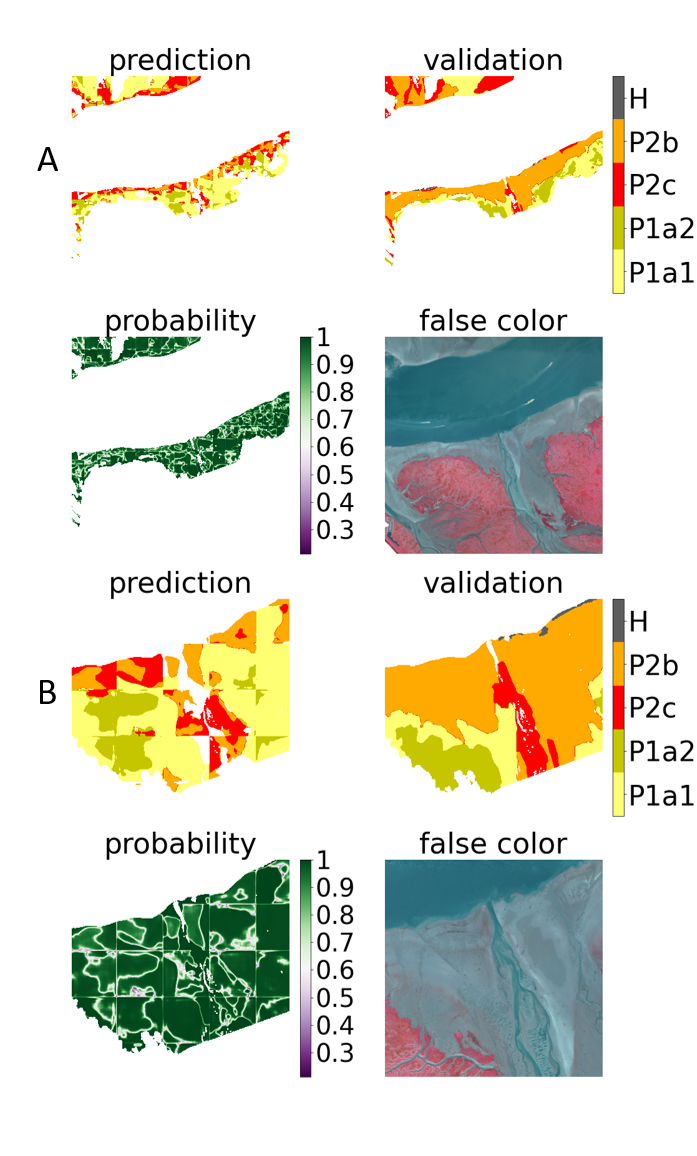
\includegraphics[scale=0.2]{figures/prediction_merged.png}
    \caption{Example of predictions from the best U-net model for Western Scheldt. A, Upper row: the prediction and the validation (i.e. reference) maps. Bottom row: the probability of the predictions and the false-color image. B, a closer look at the predictions. }
    \label{fig:deepsp}
\end{figure}

\subsubsection{Comparison between the methods OBIA-XGB and U-net}

To compare with the U-net based method, we apply the XGB model to the three tiles that are used for testing in deep learning (\cref{fig:tt}, note that these three tiles were not used in the XGB training). Comparing between \cref{tab:xgb_unettile} and \cref{deepconf}, we can observe that the OBIA-XGB method obtained a much higher accuracy. 

\begin{table}[]
    \centering
\begin{tabular}{lrrrrr}
\toprule
{} &  P1a1 &  P1a2 &  P2b &  P2c &   H1 \\
\midrule
P1a1             &  13.9 &   0.8 &  1.2 &  6.8 &  0.6 \\
P1a2             &   3.8 &  11.6 &  1.3 &  1.9 &  0.9 \\
P2b              &   8.0 &   6.4 & 15.5 &  5.1 &  2.6 \\
P2c              &   2.0 &   0.6 &  1.0 & 14.6 &  0.9 \\
H1               &   0.0 &   0.0 &  0.0 &  0.0 &  0.2 \\
precision        &  50.1 &  59.8 & 81.3 & 51.4 &  4.5 \\
recall           &  59.7 &  59.1 & 41.2 & 76.6 & 82.7 \\
overall accuracy &  55.9 &       &      &      &      \\
\bottomrule
\end{tabular}
    \caption{SSAC prediction accuracy of the OBIA-XGB method on the test tiles using in the U-net method. }
    \label{tab:xgb_unettile}
\end{table}
 
 
\section{Conclusion}

In this study, we compared machine learning methods that are based on OBIA-derived features vs. end-to-end representative learning, for inter-tidal area classification, with respectively XGBoost and U-net. The method that applies XGBoost to OBIA-derived features (OBIA-XGB) outperforms the U-net based methods. The OBIA-XGB obtained satisfying results in separating between the inter-tidal low and high dynamic shoals, as well as the natural hard substrates, which are sometimes more difficult to distinct manually or basing on the rule-based OBIA methods alone. Therefore, our study indicates that machine learning methods can help to improve the rule-based OBIA method. Future studies aim at further improvement of deep learning-based method.

%by using channel attentions, multi-scale approaches, and generative modeling. We also aim at a integration of OBIA and deep learning-based method to combine prior knowledge into machine learning techniques. Our two geomorphologically distinct study areas provide us unique opportunities to gain an in-depth insight of model generality.


\section{Acknowledgement}
 





%\bibliographystyle{plain}
\bibliography{isprs}
\end{document}

\begin{figure}[!h]
    \centering
    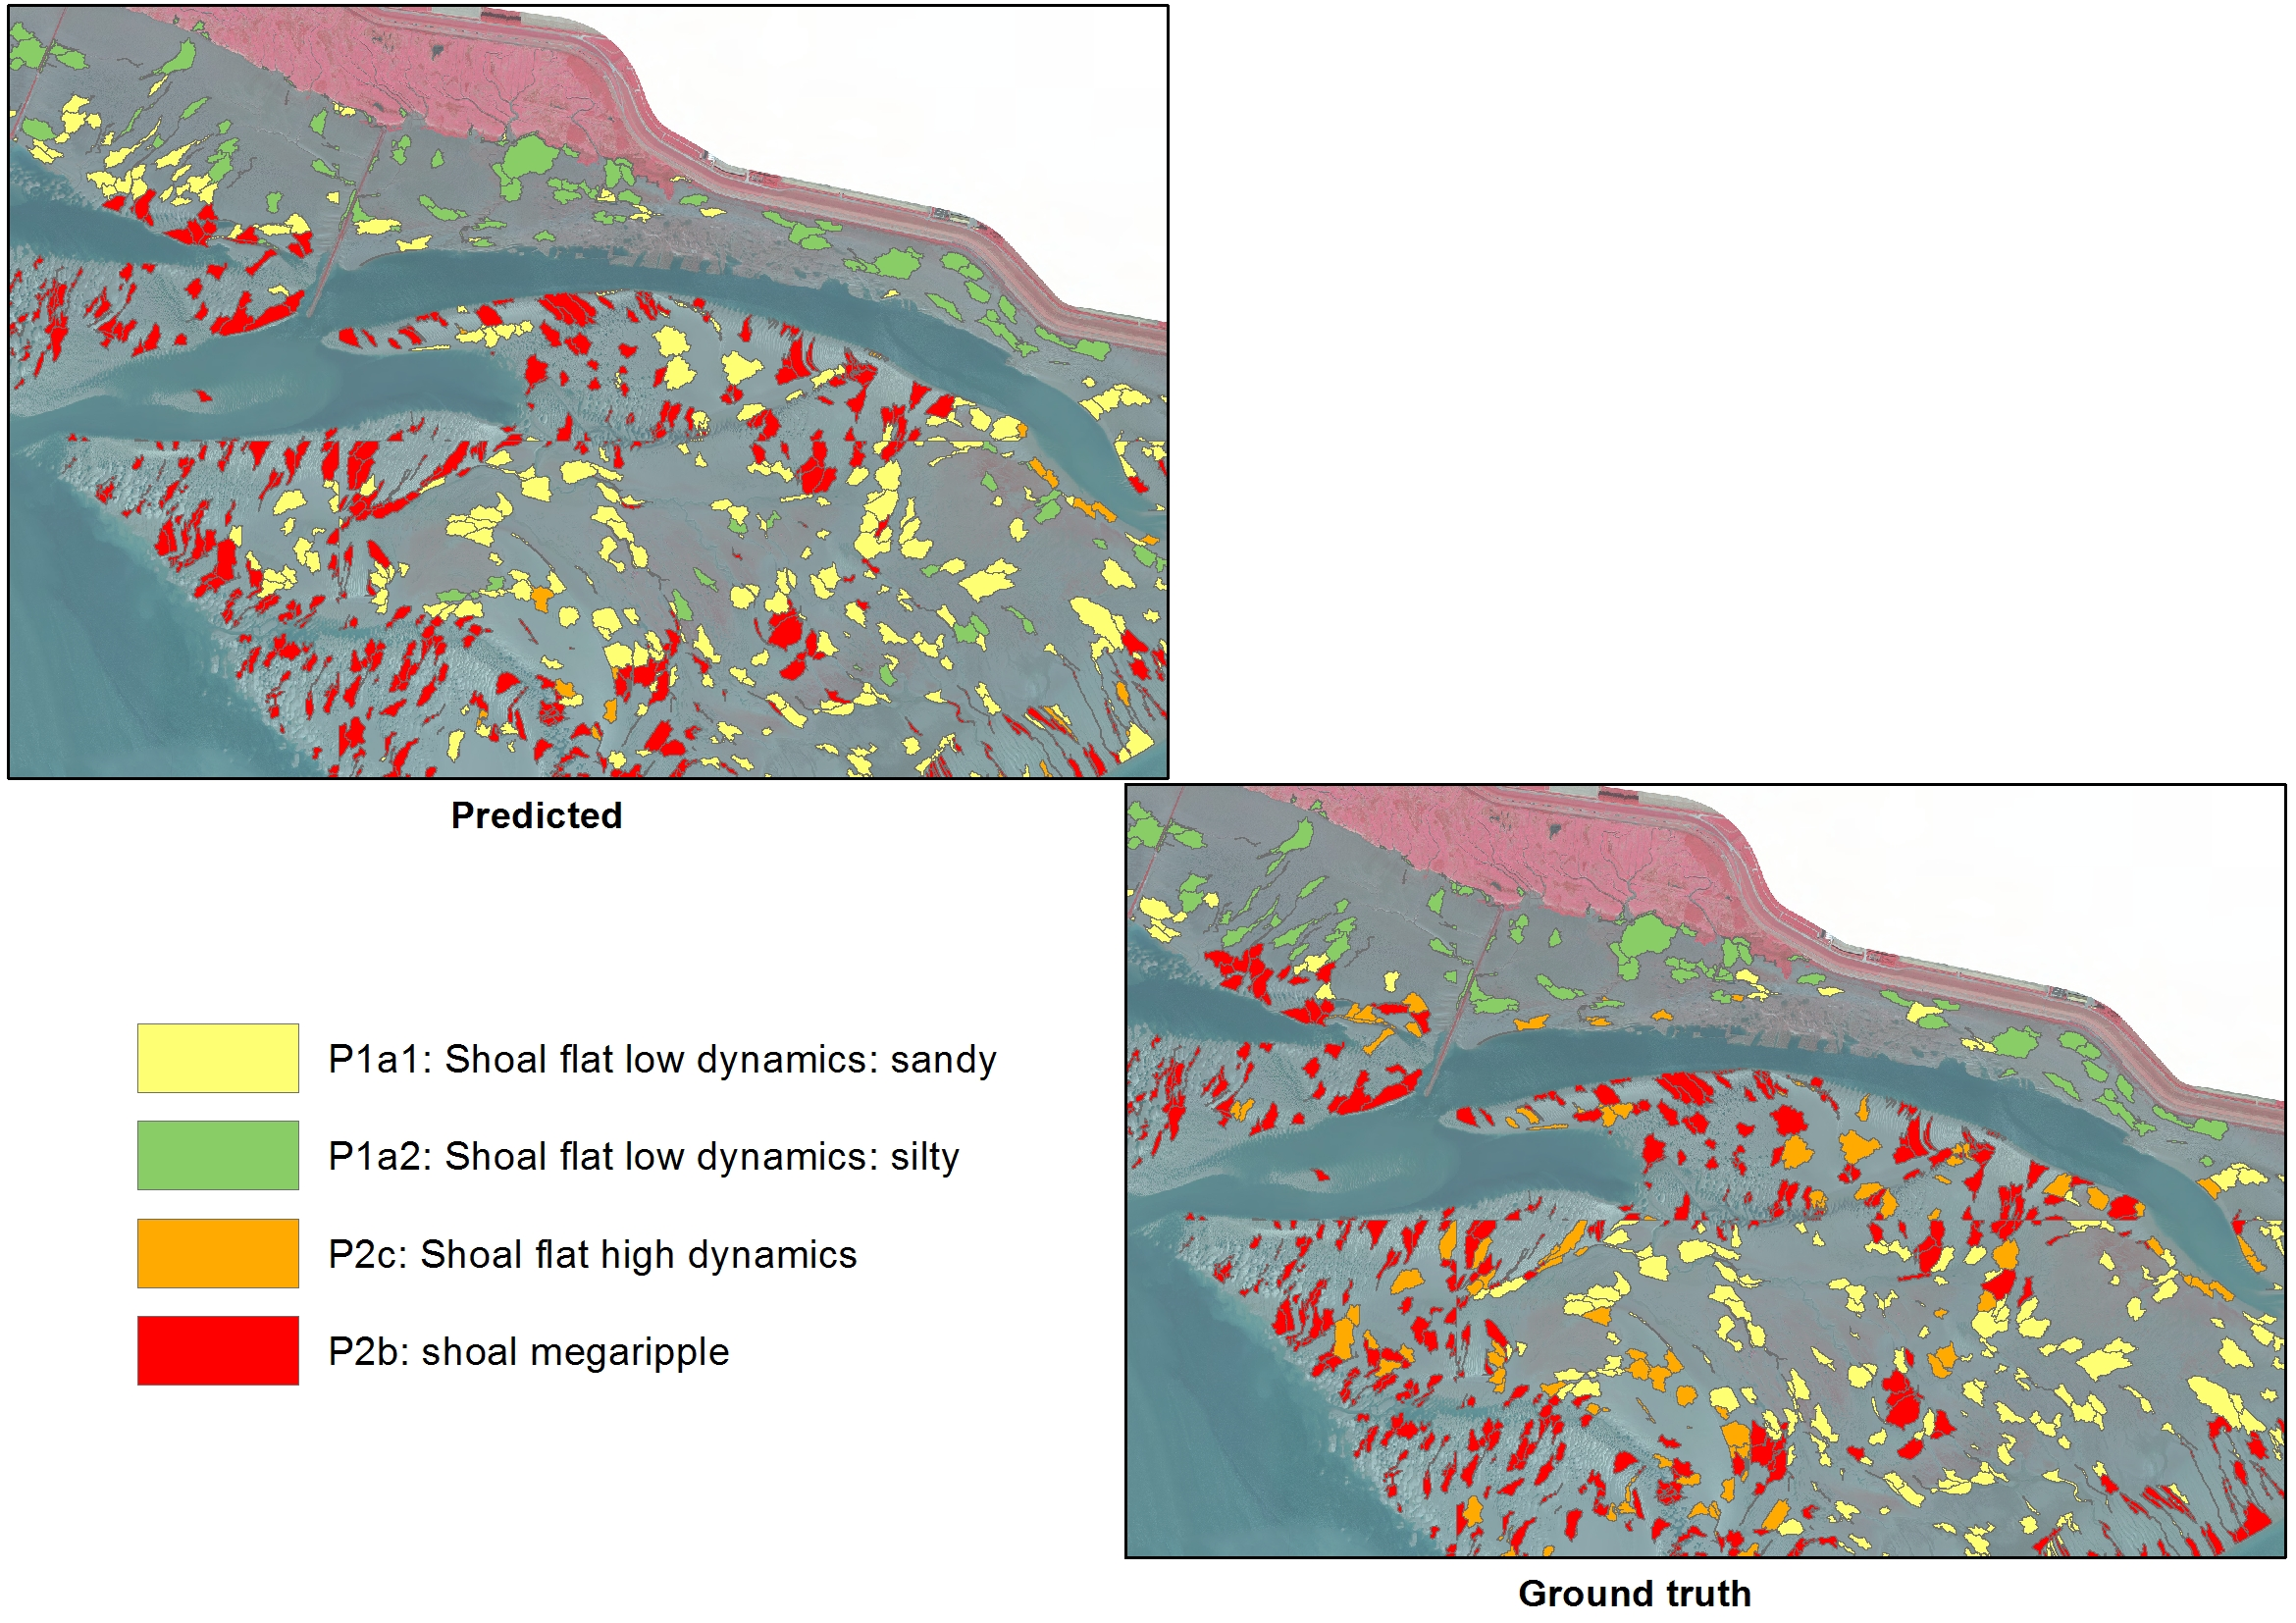
\includegraphics[scale=0.25]{figures/predictionxgb.png}
    \caption{Sampled Prediction result of four shoal classes over the test area in Western Scheldt, using the XGBboost to model the OBIA calculated object attributes.}
    \label{fig:xgb}
\end{figure}

\begin{figure}[!h]
    \centering
    \includegraphics[width=\linewidth]{figures/Spatial_50_15_P2b.png}
    \caption{Result of method A for distinguishing between mega-ripples and other classes. A: ground truth, B: predicted labels, C: prediction (in probability).}
    \label{fig:p2b}
\end{figure}